\documentclass[ngerman]{article}

% Packages
% Was macht das hier?
\usepackage[T1]{fontenc}
% Encoding der Datei (um Umlaute so zu nutzen)
\usepackage[utf8]{inputenc}
% Silbentrennung
\usepackage[ngerman]{babel}
% Für \begin{align} und Konsorten
\usepackage{amsmath}
% Für Sätze
\usepackage{amsthm}
% Für \mathbb und Konsorten
\usepackage{amssymb}
% Um im PDF geile Links zu erzeugen
% Weniger unnütze Fehlermeldungen/Warnungen hoffentlich
\usepackage{silence}
% Für internationalisierte Quotes
\usepackage{csquotes}
% Für Subfigures und Figures (alle)
\usepackage{graphicx}
\usepackage[footnotesize,bf]{caption}
\usepackage{subcaption}
% Links (und autoref)
\usepackage{hyperref}
%\def\algorithmautorefname{Algorithmus}
\addto\extrasngerman{
	  \def\algorithmautorefname{Algorithmus}
}

% Beide für Tabellen
\usepackage{array}
\usepackage{booktabs}

% Pseudocode
\usepackage{algorithmicx}
\usepackage{algorithm}
\usepackage{algpseudocode}

% Macros
\newcommand{\PimiddyName}[1]{\emph{#1}}
\newcommand{\PimiddyBegriff}[1]{\textbf{#1}}
\newcommand{\PimiddyQuotes}[1]{\enquote{#1}}
\newcommand{\PimiddyFormelText}[1]{\textrm{#1}}
\newcommand{\PimiddyReell}{\ensuremath{\mathbb{R}}}
\newcommand{\PimiddyGanz}{\ensuremath{\mathbb{Z}}}
\newcommand{\PimiddyNorm}[2]{\left\|#2\right\|_{#1}}
\newcommand{\PimiddyFootnote}[1]{\footnote{#1}}
\newcommand{\PimiddyTodo}[1]{{\tiny \textbf{TODO: #1}}}
\newcommand{\PimiddyEnglisch}[1]{{engl. \emph{#1}}}
\newcommand{\PimiddyTableHeading}[1]{{\textbf{#1}}}
\newcommand{\PimiddyInlineCode}[1]{{\texttt{#1}}}

% Operators
\DeclareMathOperator*{\PimiddyGrad}{grad}
\DeclareMathOperator*{\PimiddyDiv}{div}
\DeclareMathOperator*{\PimiddyRot}{rot}
\newcommand{\PimiddyLaplace}{\Delta}
\newcommand{\PimiddyProjection}{\mathbb{P}}
\DeclareMathOperator*{\PimiddyVectorfields}{Vect}
\DeclareMathOperator*{\PimiddyScalarfields}{Scal}

% Theorems
\newtheorem*{PimiddySatz}{Satz}

% For latex+inkscape to work. The eps_tex files use \includegraphics{foo.eps}
% which diesn't find the images unless this is defined
\graphicspath{{images/}}
% Also for latex+inkscape
\usepackage{xcolor}

\begin{document}

\section{Danksagungen}

Hiermit möchte ich allen Personen danken, die mich bei der Erstellung der Arbeit
unterstützt haben:

\begin{itemize}
\item Herrn Prof. Dr. Oliver Vornberger für die Tätigkeit als Erstgutachter und
für die Bereitstellung der interessanten Thematik.
\item Frau Prof. Dr. Sigrid Knust, die sich als Zweitgutachterin zur Verfügung gestellt hat.
\item Frau Jana Lehnfeld und Herrn Henning Wenke für das wertvolle Feedback
während der Verfassung der Arbeit.
\end{itemize}

\section{Zusammenfassung}

Die vorliegende Arbeit entstand in der Arbeitsgruppe Medieninformatik an der Universität Osna
im Bereich Computergrafik und beschäftigt sich mit prozeduraler Modellierung. Kern
der Arbeit ist die Generierung einer Schneedecke, um Wetterverhältnisse anhand
von Wetterdaten naturgetreu darstellen zu können. Dazu wird der Anzatz einer
Repräsentation durch Voxel in einem regelmaßigen Voxelgitter verfolgt. Für die
realistische Verteilung des Schnees sorgt dabei die Simulation zufalligen
Schneefalls sowie ein Stabilitatstest, der die Entstehung unnaturlich hoher
Schneeturme verhindert. Abschließend wird das Voxelgitter unter Verwendung des
sogenannten Marching-Cubes-Algorithmus' in eine schneeahnliche Oberflache
uberfuhrt.


\tableofcontents

\section{Einleitung}

\subsection{Motivation}

Die Idee, Schneefall zu modellieren, entstand im Rahmen der
Masterprojektgruppe \PimiddyQuotes{virtueller Campus} an der
Universität Osnabrück im Wintersemester 2011/12. Die Projekgruppe
befasste sich mit dem Nachbau des Campus am Westerberg der Universität
Osnabrück unter Anwendung aktueller Methoden der Computergrafik.

Die Zielsetzung der Projektgruppe enthielt auch die Visualisierung von
natürlichen Phänomenen wie einem dynamischen Wechsel von Tag und
Nacht, sowie wechselnde Wetterverhältnisse. In diesem Zusammenhang
entstand die Idee, die Modellierung von Schneefall auszulagern und
separat von der Projektgruppe zu entwickeln. Daraus entstanden zwei
Arbeiten: die vorliegende und die Bachelorarbeit von Manuel Schwarz
(\cite{Schwarz2012}).

Die Arbeit von Schwarz befasst sich mit den verschiedenen Arten, eine
dynamisch wachsende und schrumpfende, dreidimensionale Schneedecke zu
modellieren. Als Resultat wurde ein Mesh-basiertes Verfahren
implementiert, das realistische Ergebnisse mit Stabilitätsbedingungen
für den Schnee liefert. Die Visualisierung der Schneedecke stand in
dieser Arbeit allerdings nicht im Vordergrund.

Das Ziel der vorliegenden Arbeit ist die Modellierung von fallendem
Schnee, also der Bewegung von Schneeflocken im Wind. In heutigen
interaktiven Anwendungen wird meist nur der optische Eindruck von
Schneeflocken und Schneefall angenähert. In dieser Arbeit soll im
Gegensatz dazu ein Ansatz vorgestellt werden, der darauf basiert, den
Wind an sich in in Echtzeit zu modellieren und die Flocken dann anhand
des Feldes fortzutragen.

Es stellte sich die Frage, ob dies überhaupt in Echtzeit möglich sei,
oder ob die Berechnungen eher verzögert im Hintergrund ablaufen
sollten. Allerdings stellte sich heraus, dass mit der Hilfe moderner
Grafikkarten (GPUs) durchaus Echtzeitframeraten zu erreichen sind. Das
Ziel bestand darin, die entsprechenden Verfahren umzusetzen und darauf
aufbauend ein Modell für die Bewegung von Schneeflocken zu entwickeln,
welches auf das berechnete Windfeld zurückgreift.

Im Laufe der Implementierung wurde als weiteres Ziel die Integration
der Ergebnisse von \cite{Schwarz2012} hinzugefügt, um die gefallenen
Schneeflocken in die Bildung der Schneedecke einfließen zu lassen.


\subsection{Aufbau}

Da sowohl die Berechnungen für die Bewegung der Schneeflocken als auch
die strömungsmechanischen Gleichungen gewisse mathematische
Grundkenntnisse voraussetzen, werden im \autoref{sec:mathematics}
einige Mathematische Definitionen und Verfahren eingeführt. Diese
Arbeit setzt aber ansonsten keine höheren mathematischen Vorkenntnisse
voraus und sollte auch ohne Vorkenntnisse aus der Strömungsmechanik
verständlich sein.

Aufgrund der hohen Komplexität und dem Umfang des Themas ist die
Behandlung der strömungsmechanischen Zusammenhänge in drei Abschnitte
aufgeteilt. \autoref{sec:navier_stokes} gibt zunächst eine Einführung
in die Navier-Stokes-Gleichungen. Diese Gleichungen sind sehr
allgemein gefasst und beschreiben jegliche Art von Strömungen. Um die
Erklärung nicht zu kompliziert zu gestalten wird eine einfachere Form
der Gleichungen vorgestellt. Zudem werden nur die Teile näher
beleuchtet, die für die Modellierung von Wind eine Rolle spielen. Der
Abschnitt soll vor allem ein intuitives Verständnis der einzelnen
Bestandteile geben, welches für das Verständnis der Algorithmen auch
ausreichend ist.

\autoref{sec:stam} stellt das Verfahren von Stam vor. Es wird zunächst
erklärt, inwiefern sich das Verfahren von bisherigen Verfahren
unterscheidet und was es auszeichnet. Danach folgt ein allgemeiner
Überblick über die Bestandteile. Die darauf folgenden Abschnitte
erklären diese Einzelteile, wobei aber noch wenig auf eine
Implementierung eingegangen wird. Am Ende des Abschnitts sollte die
Arbeitsweise des Verfahrens klar sein, sodass es theoretisch in einer
beliebigen Programmiersprache umsetzbar wäre.

\autoref{sec:opencl} erklärt die Funktionsweise von OpenCL, wobei die
Teile nur angeschnitten werden, die für die Implementierung der
Algorithmen keine Rolle spielen. Am Ende des Abschnittes findet sich
ein simples, aber vollständiges OpenCL-Programm, welches den Ablauf
und die Interaktion zwischen GPU und CPU verdeutlicht.

In \autoref{sec:implementation_wind} wird schließlich OpenCL
eingesetzt, um das Verfahren von Stam auf die Grafikkarte zu
übertragen. Es wird viel auf \autoref{sec:stam} verwiesen und stärker
auf die Schwierigkeiten in der Implementierung eingegangen als die
Erläuterung der prinzipiellen Funktionsweise. Auch einige
Performanceoptimierungen werden angesprochen.

\autoref{sec:implementation_snowflake} widmet sich dem fallenden
Schnee. Es zunächst auf die physikalischen Ursachen für die
Entsteheung von Schnee eingangen. Danach wird die Visualisierung mit
OpenGL angesprochen. Der Rest des Abschnitts befasst sich mit den
physikalischen Besonderheiten von Schneeflocken. Als Ergebnis wird ein
OpenCL-Programm erstellt, was ein Schnee-Partikelsystem umsetzt.

\autoref{sec:fallen_snow} behandelt die Modellierung von gefallenem Schnee.

\section{Mathematische Grundlagen}

Die Berechnungen in dieser Arbeit finden alle im reellen Raum statt, also in den
Vektorräumen $\PimiddyReell^n, n \in \{1,2,3\}$. Die Gleichungen der
Strömungsmechanik benutzen \PimiddyBegriff{Vektorfelder} und
\PimiddyBegriff{Skalarfelder}, daher sollen diese Begriffe und die zugehörigen
Operationen hier eingeführt werden.

Die später betrachteten Gleichungen sind allerdings meist gar nicht oder nur sehr
schwer analytisch zu lösen, daher greift man auf numerische Verfahren zurück.
Dafür ist es allerdings notwendig, die Operationen wie den Gradienten oder die
Divergenz zu \emph{diskretisieren}. Dies kann auf verschiedene Arten geschehen,
was im letzten Teil des Abschnitts erläutert wird.

\subsection{Kontinuierliche Felder}

Für eine Funktion $f \colon \PimiddyReell^n \to \PimiddyReell$ bezeichne

\begin{equation}
\frac{\partial f}{\partial x_i}
\end{equation}

die \PimiddyBegriff{partielle Ableitung} nach der $i$-ten Komponente.

Ein \PimiddyBegriff{Vektorfeld} $\vec{u}$ ist eine Abbildung

\begin{equation*}
\vec{u} \colon \PimiddyReell^n \to \PimiddyReell^n,
\end{equation*}

die einem Punkt im Raum einen Pfeil zuordnet. So kann z.\,B. jedem Punkt im Raum
die Flussgeschwindigkeit des Fluids an diesem Punkt zugeordnet werden.
\autoref{fig:mathematics_vectorfield} zeigt ein solches Vektorfeld.
$\PimiddyVectorfields(\PimiddyReell^n)$ bezeichne die Menge aller Vektorfelder.

Analog ist ein \PimiddyBegriff{Skalarfeld} $p$ eine Abbildung

\begin{equation*}
p \colon \PimiddyReell^n \to \PimiddyReell
\end{equation*}

welche einem Punkt im Raum einen skalaren Wert zuordnet. Beispielsweise könnte
für jeden Punkt im Raum die dortige Temperatur in einem Skalarfeld gespeichert
sein (siehe \autoref{fig:mathematics_scalarfield}).
$\PimiddyScalarfields(\PimiddyReell^n)$ bezeichne die Menge aller Skalarfelder.

\begin{figure}
	\begin{subfigure}[b]{0.5\textwidth}
		\centering
		
\includegraphics[width=\textwidth]{images/vectorfield}
		\caption{Ein Vektorfeld}
		\label{fig:mathematics_vectorfield}
	\end{subfigure}
	~
	\begin{subfigure}[b]{0.5\textwidth}
		\centering
		\includegraphics[width=\textwidth]{images/thermal_imaging}
		\caption{Die Körpertemparatur eines Pferds als Skalarfeld.}
		\label{fig:mathematics_scalarfield}
	\end{subfigure}
	\caption{Die betrachteten Feldtypen}
\end{figure}

Sei $p$ ein dreidimensionales Skalarfeld, dann ist der \PimiddyBegriff{Gradient}
$\PimiddyGrad p$ definiert als:

\begin{gather}
\PimiddyGrad \colon \PimiddyScalarfields \to \PimiddyVectorfields \\
\PimiddyGrad p
=
\left( \frac{\partial p}{\partial x},\frac{\partial p}{\partial y},\frac{\partial p}{\partial z} \right)
\end{gather}

\begin{figure}[ht]
	\begin{subfigure}[b]{0.5\textwidth}
		\centering
		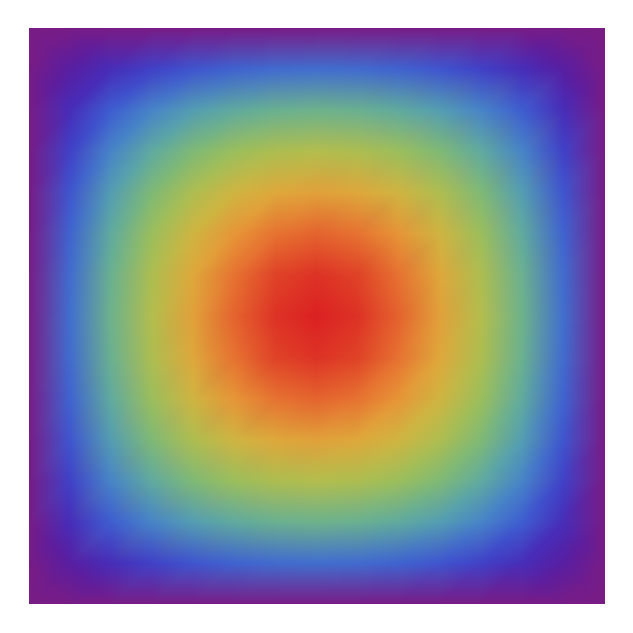
\includegraphics[width=\textwidth]{images/scalar_field_to_show_gradient}
		\caption{Das Skalarfeld zur Funktion $f(x,y) = \sin(x)\sin(y)$. Rötliche Färbung deutet hohe Werte an, lila und blau geringe.}
		\label{fig:mathematics_sample_scalar_field}
	\end{subfigure}
	~
	\begin{subfigure}[b]{0.5\textwidth}
		\centering
		
\includegraphics[width=\textwidth]{images/gradient_of_scalar_field}
		\caption{Der Gradient des Skalarfeldes $f(x,y)=(\sin(y)\cos(x),\sin(x)\cos(y))$}
		\label{fig:mathematics_gradient_of_sample_scalar_field}
	\end{subfigure}
	\caption{Der Gradient am Beispiel}
	\label{fig:mathematics_gradient_of_sample_scalar_field_total}
\end{figure}

Der Gradient eines Skalarfeldes ist also ein Vektorfeld, nämlich das Vektorfeld
der partiellen Ableitungen. Genauso wie die Ableitung eines Graphen die Steigung
an jedem Punkt angibt, so zeigt der Gradient eines Feldes in die Richtung des
steilsten Anstiegs. Seine Länge gibt die Größe Steigung an. Der Gradient des
negativen Skalarfeldes $-p$ zeigt folglich in Richtung des größten Gefälles.
\autoref{fig:mathematics_gradient_of_sample_scalar_field_total} zeigt ein simples
Beispiel für den Gradienten.

Ist ein Vektorfeld $\vec{u}$ differenzierbar (was wir in dieser Arbeit für alle
Vektorfelder annehmen), dann ist die \PimiddyBegriff{Divergenz} auf dem
Feld definiert als

\begin{gather}
\PimiddyDiv \colon \PimiddyVectorfields \to \PimiddyScalarfields \\
\PimiddyDiv \vec{u}
=
\frac{\partial u^x}{\partial x} +
\frac{\partial u^y}{\partial y} +
\frac{\partial u^z}{\partial z}
\end{gather}

Hier sind $u^x,u^y,u^z$ die einzelnen Komponenten des Vektorfeldes. Die
Divergenz eines Vektorfelds ist also ein Skalarfeld. Dieses Skalarfeld kann
gedeutet werden als \PimiddyQuotes{Quellendichte} des ursprünglichen
Vektorfeldes. Ein Feld $\vec{u}$, was $\PimiddyDiv \vec{u}=0$ erfüllt, heißt
folglich \PimiddyBegriff{quellenfrei}.

In der Physik findet man den Gradienten und die Divergenz meist unter dem Symbol
$\nabla$ vereint. Je nachdem, ob es auf ein Vektor- oder ein Skalarfeld
angewendet wird, wechselt es die Bedeutung.
%Diese Notation wird in der Arbeit bevorzugt, da man die Symbole $\PimiddyGrad$ bzw\,. $\PimiddyDiv$ in der Literatur zu Fluiddynamik kaum vorfindet.

Auf Vektorfeldern ist schließlich noch die \PimiddyBegriff{Rotation} definiert:

\begin{gather}
\PimiddyDiv \colon \PimiddyVectorfields \to \PimiddyVectorfields \\
\PimiddyDiv \vec{u}
=
\left(
	\begin{array}{c}
		\frac{\partial u^z}{\partial y} - \frac{\partial u^y}{\partial z} \\
		\frac{\partial u^x}{\partial z} - \frac{\partial u^z}{\partial x} \\
		\frac{\partial u^y}{\partial x} - \frac{\partial u^x}{\partial y}
	\end{array}
\right)
\end{gather}

Wie der Name schon andeutet gibt sie für jeden Punkt des ursprünglichen
Vektorfeldes an, wie stark und in welche Richtung das Feld in diesem Punkt
rotiert. Im Zweidimensionalen ist die Rotation auch definiert, hier ist sie
allerdings nur ein Skalar, die Rotationsachse ist immer die imaginäre
\PimiddyQuotes{$z$-Achse} (in \autoref{fig:mathematics_scalarfield} wäre die
Rotation überall konstant). Ein Feld $\vec{u}$, was $\PimiddyRot
\vec{u}=0$ erfüllt, heißt \PimiddyBegriff{rotationsfrei}.

\begin{figure}
	\begin{subfigure}[b]{0.5\textwidth}
		\centering
		\includegraphics[width=\textwidth]{images/vector_field_rotation_arrows}
		\label{fig:mathematics_image_vectorfield_rotation_arrows}
	\end{subfigure}
	~
	\begin{subfigure}[b]{0.5\textwidth}
		\centering
		\includegraphics[width=\textwidth]{images/vector_field_rotation}
	\end{subfigure}
	\caption{Ein 2D-Strömungsfeld, das um ein Hindernis herumfließt mit dazugehöriger Rotation. Negative Rotation ist rot gekennzeichnet, positive in blau.}
\end{figure}

Schaltet man $\PimiddyGrad$ und $\PimiddyDiv$ hintereinander, erhält man den
\PimiddyBegriff{Laplace-Operator}:

\begin{gather}
\PimiddyLaplace \colon \PimiddyScalarfields \to \PimiddyScalarfields \\
\PimiddyLaplace p = \PimiddyDiv \PimiddyGrad p
\end{gather}

Manchmal wird auch das Symbol $\nabla^2$ für den Laplace-Operator benutzt. Im Dreidimensionalen ergibt sich:

\begin{equation}
\PimiddyLaplace p =
\frac{\partial^2 p}{\partial^2 x} +
\frac{\partial^2 p}{\partial^2 y} +
\frac{\partial^2 p}{\partial^2 z}
\end{equation}

Intuitiv misst der Operator für jeden Punkt $\vec{x}$ die Abweichung von
$p(\vec{x})$ zu Punkten in seiner Umgebung. Die diskretisierte Variante dieses
Operators wird deswegen in der Bildverarbeitung zum Erkennen von Kanten in
Bildern verwendet (siehe \autoref{fig:mathematics_image_laplacian}).

\begin{figure}[ht]
	\begin{subfigure}[b]{0.5\textwidth}
		\centering
		\includegraphics[width=\textwidth]{images/schloss_grey}
		\caption{Originalbild}
	\end{subfigure}
	~
	\begin{subfigure}[b]{0.5\textwidth}
		\centering
		\includegraphics[width=\textwidth]{images/schloss_grey_laplace}
		\caption{Das Bild nach Anwendung des Laplace-Operators}
		\label{fig:mathematics_image_laplacian}
	\end{subfigure}
\end{figure}


Der Operator lässt sich auf nahe liegende Weise auf Vektorfelder erweitern, in drei Dimensionen
ergibt sich:

\begin{equation}
\PimiddyLaplace \vec{u} =
\left(
	\begin{array}{c}
		\PimiddyLaplace u^x \\
		\PimiddyLaplace u^y \\
		\PimiddyLaplace u^z
	\end{array}
\right)
\end{equation}

\subsection{Diskretisierung}
\label{sec:mathematics_discretization}

Die eben vorgestellten mathematischen Definitionen gehen vom unendlichen,
kontinuierlichen Raum $\PimiddyReell^n$ aus. Für die Berechnungen wird
aber ein endliches, diskretes Gitter verwendet, also eine Teilmenge von
$\PimiddyGanz^n$. Folglich müssen die Operatoren in eine diskrete Form gebracht
werden. Dies geschieht zunächst in einer Dimension.

Es sei $f \colon \PimiddyReell \to \PimiddyReell$ eine reelle Funktion, von der
wir in den späteren Berechnungen nur Stützpunkte in regelmäßigen Abständen
$\Delta x$ gegeben haben:

\begin{equation}
f_i = f(x_i) \quad , x_i = n \cdot \Delta x, n \in \PimiddyGanz
\end{equation}

Die (kontinuierliche) Ableitung dieser Funktion ist definiert als

\begin{equation}
f'(x) = \lim_{h \to 0} \frac{f(x) - f(x+h)}{x - h}
\end{equation}

Je nachdem, wie genau die Simulation sein soll, kann bei der Diskretisierung der
Ableitung unterschiedlich viel Aufwand einfließen. Grundlage für die
Diskretisierung (und die anschließende Abschätzung der Genauigkeit) ist die
\PimiddyBegriff{Taylorreihe} von $f$ (um den Entwicklungspunkt $a$):

\begin{equation}
f(x) = f(a) + f'(a)(x-a) + \frac{f''(a)}{2}(x-a)^2 + O(\Delta x^2)
\end{equation}

Nimmt man als Entwicklungspunkt $f(x_i)$ und setzt $x=x_{i+1}$ erhält man die
\PimiddyBegriff{Vorwärtsdifferenz}-Annäherung der Ableitung:

\begin{equation}
\label{eq:mathematics_forward_difference}
f'(x_i) = \frac{f(x_{i+1}) - f(x_i)}{\Delta x} + O(\Delta x)
\end{equation}

Setzt man $a=x_i,x=x_{i-1}$ erhält man analog die
\PimiddyBegriff{Rückwärtsdifferenz}:

\begin{equation}
\label{eq:mathematics_backward_difference}
f'(x_i) = \frac{f(x_i) - f(x_{i-1})}{\Delta x} + O(\Delta x)
\end{equation}

Der Nachteil dieser beiden Näherungen ist, dass sie einseitig sind (entweder
nach links oder rechts ausgerichtet) und linearen Fehler $O(\Delta x)$ haben, da
die Taylorreihe schon nach dem ersten Glied abgeschnitten wird.

Eine bessere Näherung erhält man, wenn man
\autoref{eq:mathematics_backward_difference} von
\autoref{eq:mathematics_forward_difference} subtrahiert:

\begin{equation}
f'(x_i) = \frac{f(x_{i+1}) - f(x_{i-1})}{2 \Delta x} + O(\Delta x^2)
\end{equation}

Diese Näherung wird \PimiddyBegriff{zentrale Differenz} genannt und hat
nur quadratischen Fehler $O(\Delta x^2)$. Man kann das Schema fortführen, um
noch bessere Näherung zu erhalten, dies führt allerdings dazu, dass eine immer
größere Umgebung des aktuellen Punktes betrachtet werden muss, was in der
Implementierung zu viele Speicherzugriffe verursacht.

Mit Hilfe der zentralen Differenz lässt sich auch eine Näherung für die zweite
Ableitung angeben:

\begin{equation}
f''(x_i)
=
\frac
{
	f(
		x_{i+1}) -
	2 \cdot
	f(
		x_i)
	+
	f(
		x_{i-1})
}
{
	(\Delta x)^2
}
\end{equation}

Da alle Operatoren auf partiellen Ableitungen beruhigen, lassen sich nun
diskrete Näherungen für jeden Operator angeben. Dies ist in
\autoref{table:mathematics_discrete_operator_table} für 3 Dimensionen für ein
Skalarfeld $p$ beziehungsweise ein Vektorfeld $\vec{u}$ geschehen.

\begin{table}[ht]
	\caption{Die diskretisierten Feldoperatoren in drei Dimensionen}
	\centering
	\begin{tabular}{@{}cm{10cm}@{}}
		\toprule \\

			\PimiddyTableHeading{Operator}
		&
			\PimiddyTableHeading{Diskretisierung} \\

		\midrule \\
			$\PimiddyGrad p$
		&
			\begin{equation*}
			\frac{1}{2\Delta x}
			\begin{pmatrix}
				p_{i+1,j,k} - p_{i-1,j,k}
			\\
				p_{i,j+1,k} - p_{i,j-1,k}
			\\
				p_{i,j,k+1} - p_{i,j,k-1}
			\end{pmatrix}
			\end{equation*}
		\\
			$\PimiddyDiv \vec{u}$
		&
			\begin{equation*}
			\frac
			{
				u^x_{i+1,j,k} -
				u^x_{i-1,j,k} +
				u^y_{i,j+1,k} -
				u^y_{i,j-1,k} +
				u^z_{i,j,k+1} -
				u^z_{i,j,k-1}
			}
			{
				2\Delta x
			}
			\end{equation*}
		\\
			$\PimiddyLaplace p$
		&
			\begin{equation*}
			\frac
			{
				p_{i+1,j,k} +
				p_{i-1,j,k} +
				p_{i,j+1,k} +
				p_{i,j-1,k} +
				p_{i,j,k+1} +
				p_{i,j-1,k-1} -
				6p_{i,j}
			}
			{
				(\Delta x)^2
			}
			\end{equation*}
		\\
			$\PimiddyRot \vec{u}$
		&
			\begin{equation*}
			\frac{1}{2\Delta x}
			\begin{pmatrix}
				u^z_{i,j+1,k} - u^z_{i,j-1,k} - u^y_{i,j,k+1} + u^y_{i,j,k-1}
			\\
				u^x_{i,j,k+1} - u^x_{i,j,k+1} - u^z_{i+1,j,k} + u^z_{i,j,k-1}
			\\
				u^y_{i+1,j,k} - u^y_{i-1,j,k+1} - u^x_{i,j+1,k} + u^x_{i,j-1,k}
			\end{pmatrix}
			\end{equation*}
		\\
		\bottomrule
	\end{tabular}
	\label{table:mathematics_discrete_operator_table}
\end{table}

\section{Die Navier-Stokes-Gleichungen}
\label{sec:navier_stokes}

\subsection{Fluide}

Die Gleichungen, die im folgenden beschrieben werden, gelten nicht nur
für Gase wie Luft, sondern auch für Flüssigkeiten wie Wasser. Deshalb
wird im Folgenden der Begriff \PimiddyBegriff{Fluid} verwendet,
welcher beide Zustände zusammenfasst. Physikalisch gesehen sind
Fluide Substanzen, die einer beliebig langsamen Scherung keinen
Widerstand entgegensetzen. Dieses Konzept ist allerdings in dieser
Arbeit nicht von Bedeutung.

Welches Modell man für die Bewegung von Fluiden wählt, hängt davon ab,
welche Art von Fluid man modelliert. Bei dickflüssigen Fluiden wie
Honig muss ein Modell gewählt werden, was die Viskosität gut
modelliert. Bei Fluiden mit geringer Dichte wie Luft können dagegen
einige Faktoren ausgelassen werden. Auch die äußeren Gegebenheiten
haben Einfluss auf das Modell. Daher sollen zunächst die
Rahmenbedingungen des Modells erläutert werden, bevor die zugehörigen
Gleichungen vorgestellt werden.

Das \emph{Volumen} von Fluiden ist im Allgemeinen nicht konstant, es
wird durch Veränderung von Druck und Dichte beeinflusst. Dies
geschieht z.\,B.\ beim Übertreten der Schallmauer (im Medium Luft,
beispielsweise bei einer Explosion) oder bei der Ausbreitung von Tönen
unter Wasser. In der Strömungsmechanik unterscheidet man daher
zwischen \PimiddyBegriff{komprimierbaren} und
\PimiddyBegriff{unkomprimierbaren} Fluiden, je nachdem, ob die
Veränderung des Volumens eine Rolle für die Simulation spielt.

Es werden hier nur \emph{unkomprimierbare} Fluide betrachtet. Dies
stellt kein Problem dar, da nur vergleichsweise kleine
Geschwindigkeiten betrachtet werden.  Das Modell wird dadurch
allerdings wesentlich vereinfacht.

Zudem haben Fluide im allgemeinen an jedem Punkt $\vec{x}$ eine
unterschiedliche \emph{Dichte} $\rho(\vec{x})$. Diese wird im
Wesentlichen von Druck und Temperatur beeinflusst. Zur weiteren
Vereinfachung wird hier allerdings von einer konstanten Dichte $\rho$
ausgegangen und beispielsweise die Temperatur nicht in die
Betrachtungen einbezogen. Effekte wie Auftrieb durch
Temperaturunterschiede können allerdings optional in das Modell
eingepasst werden, siehe \autoref{sec:stam_buoyancy}.

\subsection{Einführung}

Das Modell eines Fluids besteht mathematisch gesehen aus mehreren Feldern
(Skalar- und Vektorfeldern), die den Zustand des Fluids zu einem
\emph{Zeitpunkt} $t$ an einer \emph{Position} $\vec{x}$ angeben.

In den \PimiddyBegriff{Navier-Stokes-Gleichungen}, die in
\autoref{eq:navier_stokes_equation} dargestellt sind, werden zwei
Felder betrachtet, die \emph{Bewegungsgeschwindigkeit}
$\vec{u}(\vec{x},t)$ des Fluids und der \emph{Druck}
$p(\vec{x},t)$. Die Gleichungen wurden 1822 von
\PimiddyName{Claude-Louis Navier} und 1845 von \PimiddyName{George
Gabriel Stokes} formuliert\cite{Muller2003}.

\begin{figure}
\begin{align}
\label{eq:navier_stokes_momentum_equation}
\frac{
	\partial
	\vec{u}
}
{
	\partial t
} +
\vec{u} \PimiddyDiv \vec{u}
& =
\vec{g} +
\nu \PimiddyLaplace \vec{u} -
\frac{
	1
}
{
	\rho
}
\PimiddyGrad p
\\
\label{eq:navier_stokes_incompressibility_condition}
\PimiddyDiv \vec{u} & = 0
\end{align}
\caption{Die unkomprimierbaren Navier-Stokes-Gleichungen}
\label{eq:navier_stokes_equation}
\end{figure}

\autoref{eq:navier_stokes_momentum_equation} ist eine Differentialgleichung, die
wegen des Terms $\vec{u} \PimiddyDiv \vec{u}$ nichtlinear ist. Das macht sie
besonders schwer mit klassischen Verfahren lösbar.

Die Dimension des Raums taucht in den Gleichungen nicht auf, man kann sie also
in zwei oder drei Dimensionen betrachten. Zur Veranschaulichung wird im
Folgenden oft von zwei Dimensionen ausgegangen.

Die einzelnen Bestandteile werden in den folgenden Kapiteln genauer beleuchtet,
hier soll allerdings schon ein kurzer Überblick gegeben werden:

\begin{itemize}
\item
	Die Konstante $\rho$ gibt die \emph{Dichte} des Fluids an. Für Wasser beträgt
	sie etwa $1000 \frac{kg}{m^3}$, für Luft etwa $1.3
        \frac{kg}{m^3}$ \cite{Bridson2007}.
\item
	Der \emph{Druck} $p$ spielt bei den späteren Berechnungen eine große Rolle.
	Er ist dort besonders hoch, wo das Fluid auf Hindernisse
        trifft und diese umfließt.
\item
	Kräfte, die von außen auf das Fluid wirken, wie z.\,B.\ die Schwerkraft
	oder auch der eingeführte Wind, werden im Vektorfeld $\vec{g} \colon
	\PimiddyReell^3 \to \PimiddyReell^3$ zusammengefasst.
\item
	Fluide unterscheiden sich in ihrer \PimiddyBegriff{Viskosität}
	oder \PimiddyQuotes{Zähflüssigkeit}, die in der Gleichung mit $\nu$
	bezeichnet ist. Dickflüssige Fluide wie Honig haben ein hohes $\nu$,
	dünnflüssige wie Luft ein niedriges $\nu$.
\end{itemize}

\autoref{eq:navier_stokes_momentum_equation} wird
\PimiddyBegriff{Impulsgleichung} genannt,
\autoref{eq:navier_stokes_incompressibility_condition} nennt man
\PimiddyBegriff{Unkomprimierbarkeitsbedingung}. Der Name und die Bedeutung der
Gleichungen werden im Folgenden näher beleuchtet.

Die Navier-Stokes-Gleichungen komplett zu erläutern geht über den Rahmen dieser
Arbeit weit hinaus, daher soll vor allem ein intuitives Verständnis der
einzelnen Bestandteile gegeben werden. Außerdem soll eine Beziehung zur
klassischen Mechanik hergestellt werden, da die Gleichungen starke Parallelen
hierzu aufweisen.

\subsection{Die Impulsgleichung}

\subsubsection{Lagrange und Euler}

Um Fluide zu modellieren, gibt es zwei Betrachtungsweisen. Die
\PimiddyBegriff{Euler'sche-Be\-trach\-tungs\-wei\-se} und die
\PimiddyBegriff{Lagrange'sche-Betrachtungsweise}.

Bei der \emph{Lagrange'schen-Betrachtungsweise} modelliert man das
Fluid als System von mikroskopisch kleinen \emph{Partikeln} (man
modelliert sozusagen die Moleküle des Fluids einzeln). Jedes Partikel
hat ein Volumen $V$, eine Masse $m$, eine Position $\vec{x}$ und eine
Geschwindigkeit $\vec{u}$. In jedem Simulationsschritt berechnet man
die Kräfte, die auf die Partikel wirken, und berechnet die
resultierende Beschleunigung mit der Newton'schen Formel:

\begin{align*}
m \cdot \vec{a} &= \vec{F} \\
m \cdot \frac{\partial \vec{u}}{\partial t} &= \vec{F}
\end{align*}

Diese Vorgehensweise ist intuitiv und einfach umzusetzen, aber mathematisch
schwer zu analysieren. Beispielsweise kann man die Frage \PimiddyQuotes{Welche
Geschwindigkeit hat das Fluid an Position $\vec{x}$?} nicht sofort
beantworten. Bei der Bewegung der Schneeflocken ist dies aber äußerst
wichtig.

Bei der \emph{Euler'schen-Betrachtungsweise} hingegen hält man jeweils einen Punkt im
Raum fest und analysiert das Strömungsverhalten (Geschwindigkeit, Temperatur)
durch diesen Punkt. Diese Art der Modellierung ist weniger intuitiv, lässt sich
mit Hilfe von Vektorfeldern und Skalarfeldern aber sehr gut mathematisch erfassen.

\subsubsection{Die substantielle Ableitung}

\begin{figure}[ht]
\centering
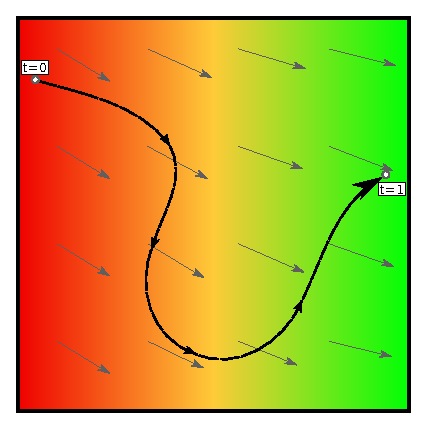
\includegraphics[width=8cm]{images/swimmer_in_water}
\caption{Die Bahn eines Bootes im Wasser. Die Temperatur des Fluids ist hier durch Farben kodiert. Rot bedeutet warmes Wasser, grün bedeutet kaltes Wasser. Nicht dargestellt ist die Veränderung der Wassertemperatur über die Zeit.}
\end{figure}

Sowohl die Euler'sche- als auch die Lagrang'sche Betrachtungsweise spiegeln sich
in den Navier-Stokes-Gleichungen wider. Obwohl es nicht sofort
erkennbar ist, bilden die Gleichungen eine Entsprechung der Gleichung
$\vec{F} = m \cdot \vec{a}$ mit dem Unterschied, dass keine Kraft auf
einen einzelnen Körper berechnet wird, sondern auf einen ganzen
Raumabschnitt (ein \PimiddyQuotes{Kontinuum}).

Was die beiden Betrachtungsweisen verbindet, ist die
\PimiddyBegriff{substantielle Ableitung}. Zur Herleitung dieser
Ableitungsform betrachten wir zunächst eine beliebige Größe
$q(\vec{x},t)$. Dies kann eine skalare Größe wie z.\,B.\ die Temperatur
eines Gewässers sein oder eine Vektorgröße wie die Farbe des Wassers
an einem Punkt. Da $q$ in jedem Punkt definiert ist, stellt die
Funktion eine Euler'sche Größe dar.

Zudem betrachten wir ein Partikel mit einer Bewegungsbahn durch das
Fluid (z.\,B.\  ein Ruderboot im Wasser). Seine Position zum Zeitpunkt
$t$ sei gegeben durch $\vec{p}(t)$. Dies entspricht einer
Lagrange'schen Größe.

Setzen wir beide Größen zusammen, erhalten wir beispielsweise die
Temperatur des Wassers auf der Bahn, die das Boot im Wasser verfolgt:

\begin{equation}
\PimiddyFormelText{Temperatur}(t) = q(\vec{p}(t),t)
\end{equation}

Wollen wir wissen, wie sich die Umgebungstemperatur des Bootes im Lauf
der Zeit verändert, bilden wir die (totale) Ableitung dieser
zusammengesetzten Größe:

\begin{equation}
\frac{
	\partial \PimiddyFormelText{Temperatur}(t)
}
{
	\partial t
}
=
\frac{
	\partial q
}
{
	\partial t
}
+
\PimiddyGrad q \cdot
\frac{
	\partial \vec{p}}
{
	\partial t
}
\end{equation}

Die Summe auf der rechten Seite besteht aus zwei Teilen. Der erste Term,
$\frac{\partial q}{\partial t}$, gibt an, wie sich das Fluid unabhängig von
der betrachteten Position verändert. Bezogen auf das Boot gibt dieser
Term an, wie sich die Temperatur des Gewässers über den Tag verteilt
verändert, beispielsweise durch den Einfluss der Sonnenstrahlen. Der
zweite Term ergänzt die globale Ableitung durch die lokale
Temperaturänderung, die durch die Bahn des Bootes verursacht
wird.

Statt eines beliebigen Pfades durch das Fluid nimmt man zur Definition der
substantiellen Ableitung nun das Geschwindigkeitsfeld des Fluids zur Hilfe:

\begin{equation}
\frac{
	Dq}
{
	Dt
} :=
\frac{
	\partial q
}
{
	\partial t
}
+
\PimiddyGrad q \cdot
\vec{u}
\end{equation}

Man geht also von einem Partikel aus, was sich im Fluid \PimiddyQuotes{treiben}
lässt, und misst die Veränderung der Größe $q$ auf seiner Bahn. Analog ist die
substantielle Ableitung für Vektorgrößen definiert:

\begin{equation}
\frac{
	D\vec{q}}
{
	Dt
} :=
\frac{
	\partial q
}
{
	\partial t
}
+
\PimiddyDiv q \cdot
\vec{u}
\end{equation}

Die Impulsgleichung lässt sich mit Hilfe der substantiellen Ableitung so schreiben:

\begin{equation}
\rho \frac{D\vec{u}}{Dt} = - \PimiddyGrad p + \PimiddyLaplace \vec{u} + \vec{f}
\end{equation}

Dies entspricht der klassischen Newton'schen Kraftformel, wobei die
Masse $m$ durch die Dichte $\rho$ ersetzt wird. Auf der rechten Seite
der Gleichung stehen die Kräfte, die das Fluid beeinflussen. Diese
Kräfte sollen im Einzelnen näher beschrieben werden.

\subsubsection{Die Kräfte in den Navier-Stokes-Gleichungen}

Die Kraft, die überall im Fluid in gleicher Weise wirkt, ist die Schwerkraft:

\begin{equation}
F_g =
\left(
\begin{array}{c}
0 \\
-g \\
0
\end{array}
\right)
\end{equation}

mit $g \cong 9.81 \frac{m}{s^2}$.

Durch den Druck $p$ des Fluids wird eine weitere Kraft $F_p$ ausgeübt.
Allerdings erzeugt die Anwesenheit von Druck (also $p \neq 0$) allein
keine Kraft. Ist der Druck beispielsweise im gesamten Fluid konstant,
ist die ausgeübte Kraft gleich 0. Stattdessen wirkt $F_p$
\PimiddyQuotes{ausgleichend}. Sie zeigt von Bereichen hohen Drucks hin
zu Bereichen niedrigeren Drucks. Mathematisch gesehen ist $F_p$ also
proportional zum negativen Gradient des Drucks.

\begin{equation}
\label{eq:navier_stokes_f_p}
F_p = -\PimiddyGrad p
\end{equation}

 In \autoref{fig:navier_stokes_particle_system_wall_collision}) ist
dies intuitiv anhand eines Partikelsystems erläutert. Treffen die
Partikel auf eine Wand, entsteht Druck, der tangential zur Wand wirkt
und die Partikel in diese Richtung beschleunigt. In den späteren
Berechnungen spielt der Druck insbesondere eine Rolle, um das Fluid in
seinem unkomprimierbaren Zustand zu halten und um das Hineinfließen in
Hindernisse zu verhindern.

\begin{figure}[ht]
\centering
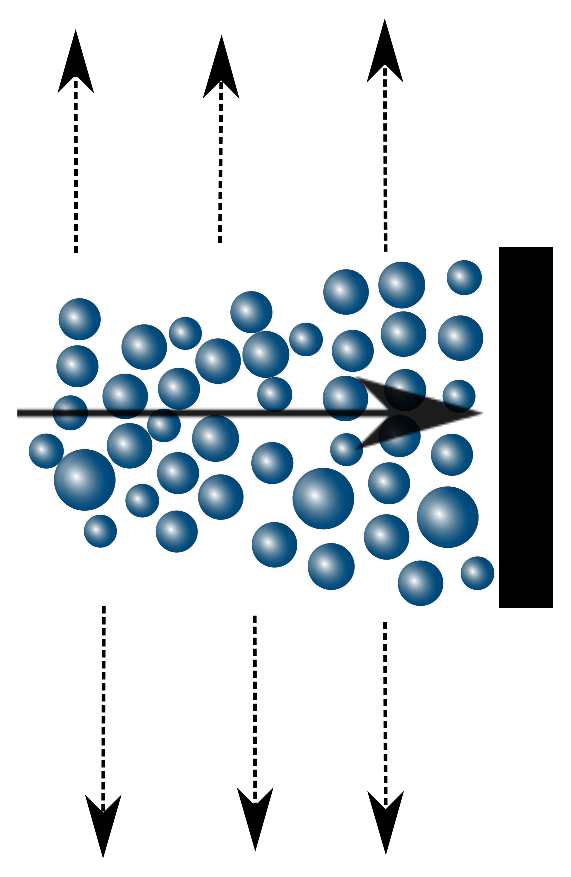
\includegraphics[width=6cm]{images/particle_system_wall_collision}
\caption{Partikelsystem, das auf ein Hindernis prallt. Der durchgezogene Pfeil deutet die Fließrichtung an, die gestrichelten Pfeile den negativen Gradienten des Drucks. Die Partikel erfahren also eine Kraft nach außen.}
\label{fig:navier_stokes_particle_system_wall_collision}
\end{figure}

Die Viskosität des Fluids hat ebenfalls Einfluss auf das Fluid. Bei einem
viskosen Fluid wird jeder Deformation ein Widerstand entgegengesetzt. Eine
Flüssigkeit wie Honig, die um ein Hindernis herumfließt, bildet hinter dem
Hindernis keine Verwirbelungen; die hohe Viskosität wirkt dem entgegen. Luft
hingegen hat eine niedrige Viskosität, bildet also besonders viele Wirbel.

Die Kraft, die durch die Viskosität ausgeübt wird, hat den Effekt,
Geschwindigkeitsunterschiede innerhalb des Fluids auszugleichen. Sie ist
daher proportional zum Laplace der Geschwindigkeit:

\begin{equation}
\label{eq:navier_stokes_f_v}
F_v = \mu \cdot \PimiddyLaplace \vec{u}
\end{equation}

Die Konstante $\mu$ stellt die \PimiddyBegriff{dynamische Viskosität}
des Fluids dar.

\subsection{Die Unkomprimierbarkeitsbedingung}
\label{sec:mathematics_incompressibility_condition_section}

\begin{figure}[ht]
\centering
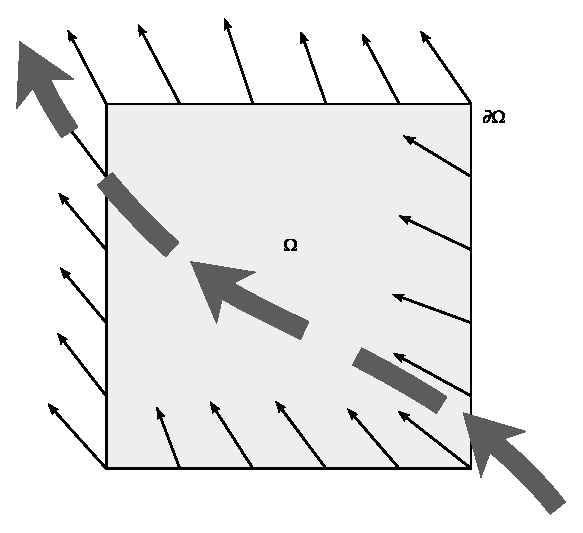
\includegraphics[width=10cm]{images/incompressibility_condition_example}
\caption{Fluss durch ein Rechteck. Der große Pfeil deutet die Fließrichtung des Fluids an. Die Pfeile an den Rändern des Rechtecks zeigen in die dortige Fließgeschwindigkeit, über deren Normalenkomponente in \autoref{eq:navier_stokes_incompressibility_initial_integral} integriert wird.}
\label{fig:navier_stokes_incompressibility_condition_example}
\end{figure}

Um die Unkomprimierbarkeitsbedingung zu motivieren, sei ein beliebiges Volumen
$\Omega \subset \PimiddyReell^3$ gegeben, \PimiddyzB ein Würfel im Raum. Seine
Oberfläche sei $\partial \Omega$.

Die Änderung des Würfelvolumens über die Zeit kann berechnet werden,
indem man über die Normalenkomponente entlang seiner Oberfläche
integriert \cite{Chorin1980}. Bildlich gesprochen summiert man auf
diese Weise eingehende und ausgehende Strömungen an den
Würfelseitenflächen (\Pimiddyvgl
\autoref{fig:navier_stokes_incompressibility_condition_example}):
\begin{equation}
\label{eq:navier_stokes_incompressibility_initial_integral}
\frac{
	\partial \PimiddyFormelText{Volumen}(\Omega)
}
{
	\partial t
}
=
\iint_{\partial \Omega} \vec{u} \cdot \vec{n}
\end{equation}
Damit die Flüssigkeit unkomprimierbar ist -- sich das Volumen also
nicht ändert -- sollte dieses Integral verschwinden:
\begin{equation}
\iint_{\partial \Omega} \vec{u} \cdot \vec{n} = 0
\end{equation}
Mit Hilfe des Divergenzsatzes können wir dieses Integral in ein Volumenintegral
umformen:
\begin{equation}
\iiint_\Omega \PimiddyDiv \vec{u} = 0
\end{equation}
Da $\Omega$ beliebig gewählt war, folgt die
Unkomprimierbarkeitsbedingung $\PimiddyDiv \vec{u} = 0$.

\section{Methode nach Stam}

\subsection{Motivation}

Die Methode zur approximativen Lösung der Navier-Stokes-Gleichungen, die im
Folgenden erklärt wird, wurde von \PimiddyName{Jos Stam} im Jahr 1999 entwickelt
und in dem Paper "`Stable Fluids"' vorgestellt \cite{Stam1999}. Das Verfahren
wurde speziell für die Computergrafik entwickelt, wobei auf einige
Besonderheiten eingegangen wurde:

\begin{enumerate}
\item
	Im Gegensatz zu wissenschaftlichen Simulationen ist man in der
	Computergrafik an einer Lösung interessiert, die in möglichst kurzen
	Abständen Ergebnisse produziert. Zum Beispiel möchte man die
	Strömungssimulation jedes Frame um einen Zeitschritt weiterbewegen. Um
	eine flüssige Simulation zu erhalten, ist die Laufzeit des
	Lösungsalgorithmus also auf 16 Millisekunden (für 60 Bilder pro Sekunde)
	bzw. 33 Millisekunden (für 30 Bilder pro Sekunde) beschränkt. Die
	Navier-Stokes-Gleichungen bilden als System von nichtlinearen
	Differentialgleichungen hier eine besondere Herausforderung.
\item
	Man ist außerdem nicht unbedingt an einer exakten Lösung interessiert.
	Will man z.B. Wasser oder Rauch simulieren reicht es, ein physikalisch
	annähernd korrektes Verhalten zu erzielen.
\item
	Bisherige Verfahren (wie z.B. die finiten Differenzen in
	\cite{Foster1997}) waren numerisch \emph{instabil} für große
	Zeitschritte. Dynamische Anwendungen wie Spiele oder Animationssoftware
	können allerdings keine minimiale Framerate garantieren, da sie mit
	verschiedenen Umgebungen und Hardwarekonfigurationen ausgeführt werden
	können.

	Als Ausweg muss man einen großen Zeitschritt (ein langes Frame) entweder
	ignorieren -- was die Simulation unrealistisch macht -- oder ihn in
	kleinere Zeitschritte unterteilen. Die Laufzeit des Verfahrens ist aber
	im Allgemeinen nicht von der Größe des Zeitschritts abhängig. Dies führt
	dazu, dass das nächste Frame erneut viel Rechenzeit benötigt und wieder
	entsprechend lang wird.

	Dieser Effekt ist nicht mehr aufzuhalten und die Simulation
	\PimiddyQuotes{explodiert}.
\item
	Bisherige Verfahren waren auf Hilfe des Designers angewiesen, um Teile
	der Simulation möglichst realistisch zu modellieren. Bestimmte natürlich
	vorkommende Turbulenzen mussten explizit in die Simulation eingegeben
	werden. Idealerweise sollte die Simulation allerdings von selber
	fortgeführt werden, der Designer sollte nur Rahmenbedingungen wie
	Hindernisse und globale Eigenschaften des Fluids (wie Dichte und
	Viskosität) vorgeben.
\end{enumerate}

\begin{figure}[ht]
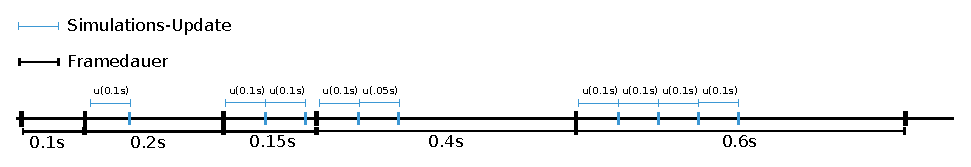
\includegraphics[width=12cm]{images/simulation_blowup}
\caption{Instabilität in Simulationen: Hier wird angenommen, die maximal zu simulierende Simulationsdauer sei $0.1s$. Längere Frames werden in mehreren Ticks berechnet, die aber konstant lange Laufzeit haben. Dies führt zu dauerhaft langen Frames, der Effekt potenziert sich.}
\end{figure}

Das Verfahren ist also auf Geschwindigkeit ausgelegt, basiert aber
nichtsdestotrotz auf den Navier-Stokes-Gleichungen und erzielt akkurate
Simulationsergebnisse. Anfängliche Schwachstellen des Verfahrens wie die zu
starke Dämpfung von Wirbeln wurden in weiteren Arbeiten ausgebessert
\cite{Foster}. Diese Verbesserungen sind teilweise auch in die Arbeit
eingeflossen.

Wegen der numerischen Stabilität und sehr guten Parallelisierbarkeit wird Stams
Verfahren bereits in einigen Spielen eingesetzt (siehe \cite{Crane2007},
\cite{Peschel2009}). Hier beschrieben wird eine leicht abgewandelte
Fassung, bei der andere Randbedingungen verwendet werden.

\subsection{Überblick über das Verfahren}

Die Fluidsimulation findet auf einem kollokierten Gitter statt.

Die Fluidsimulation findet auf einem diskreten, endlichen Gitter, also einer
Teilmenge von $\PimiddyGanz^n$ statt. Gegeben sei ein anfängliches Strömungsfeld
$\vec{u}$. In diesem Feld könnten z.B. alle Geschwindigkeitsvektoren auf eine
vorgegebene \PimiddyQuotes{Windrichtung} gesetzt sein. Gegeben sei außerdem ein
Zeitdelta $\Delta t$ (nicht zu verwechseln mit dem Laplaceoperator). Ziel ist
es, das Feld unter Zuhilfenahme der Navier-Stokes-Gleichungen einen diskreten
Zeitschritt weiter zu bewegen.

Die rechte Seite Impulsgleichung \eqref{navier_stokes_momentum_equation} besteht
aus mehreren Summanden:

\begin{equation}
\vec{g} +
\nu \PimiddyLaplace \vec{u} -
\vec{u} \PimiddyDiv \vec{u} -
\frac{
	1
}
{
	\rho
}
\PimiddyGrad p
\end{equation}

Jeder dieser Summanden stellt eine Operation dar, die
separat behandelt werden kann:

\begin{itemize}
\item
	Der Term $\vec{g}$ umfasst schlicht das Aufsummieren aller äußeren
	Kräfte, die auf das Fluid wirken. Hierzu gehört sowohl die Schwerkraft
	als auch der von außen eingeführte Wind.
\item
	Der Term
	\begin{equation}
	\nu \PimiddyLaplace \vec{u}
	\end{equation}
	stellt die viskose \PimiddyBegriff{Diffusion} dar. Selbst wenn keine
	Kräfte auf das Fluid wirken, bewegt es sich durch Diffusionsprozesse
	weiter, so wie Farbe auf einem Blatt Papier verläuft.

	Dieser Term kann in Stams Verfahren ignoriert werden, er entsteht
	ohnehin durch Genauigkeitsfehler während der Advektion (siehe unten). So
	kann Performance eingespart werden, denn die Lösung dieses Terms ist
	sehr aufwändig.
\item
	Der Term
	\begin{equation}
	\vec{u} \PimiddyDiv \vec{u}
	\end{equation}
	stellt die \PimiddyBegriff{Advektion} dar. Das Vektorfeld wird entlang
	seiner eigenen Strömungsrichtung weiterbewegt.
\item
	Der \emph{Druck} des Fluids wird in dem Term
	\begin{equation}
	\frac{1}{\rho} \PimiddyGrad p
	\end{equation}
	zusammengefasst. Er dient später dazu, die Randbedingungen und die
	Unkomprimierbarkeit zu erzwingen.
\item
	Wie bei Differentialgleichungen üblich, müssen wir noch die
	\emph{Randbedingungen} behandeln.
\end{itemize}

\begin{figure}[ht]
\includegraphics[width=10cm]{images/stam_loop}
\caption{Die Simulationsschleife ohne Projektion.}
\end{figure}

Für jeden Term wird im Folgenden ein Lösungsalgorithmus vorgestellt. Allerdings
garantiert keiner dieser Algorithmen, dass das Fluid nach Anwendung noch
unkomprimierbar ist. Die zweite Bedingung
\ref{navier_stokes_incompressibility_condition} kann also verletzt sein, und
unsere Simulation ist nicht mehr akkurat.

Gesucht ist ein Operator $\PimiddyProjection$, der ein Vektorfeld auf ein
quellenfreies Vektorfeld abbildet. Hierzu bedient man sich eines Ergebnisses aus
der Vektoranalysis, der \PimiddyBegriff{Helmholtz-Zerlegung} (auch
Helmholtz-Hodge-Theorem oder Ladyzhenskaya-Theorem genannt): Sei $\vec{u}$ ein
zweimal stetig differenzierbares Vektorfeld auf
einem beschränkten Definitionsbereich, dann lässt $\vec{u}$ sich zerlegen in ein
\emph{quellenfreies} Vektorfeld $\vec{w}$ und den \emph{Gradienten} eines
Skalarfeldes $p$:

\begin{equation}
\vec{u} = \vec{w} + \PimiddyGrad p
\end{equation}

Diese Gleichung wollen wir nach $\vec{w}$ auflösen und dieses Feld dann für die
weiteren Schritte verwenden. Dazu wenden wir die Divergenz auf die Gleichung an
und nutzen aus, dass der Operator linear ist:

\begin{equation}
\PimiddyDiv \vec{u} = \PimiddyLaplace p
\end{equation}

Dies ist eine sogenannte \PimiddyBegriff{Poissongleichung}, und ihre Lösung ist
ein Standardproblem in der Physik. Es wird später ein Verfahren vorgestellt, was
die obige Gleichung nach $p$ auflösen kann. Damit können wir dann durch
Umstellen und Bildung des Gradienten $\vec{w}$ bestimmen:

\begin{equation}
\vec{w} = u - \PimiddyGrad p
\end{equation}

Wir definieren jetzt

\begin{equation}
\PimiddyProjection \colon \PimiddyReell^n \to \PimiddyReell^n
\end{equation}

als die Funktion, die ein Vektorfeld auf den quellenfreien Anteil der
Helmholtz-Zerlegung abbildet (ein Vektorfeld also quellenfrei
\PimiddyQuotes{macht}). Führt man diesen nach der Advektion aus, erhält man eine
stabile Simulation.

\begin{figure}[ht]
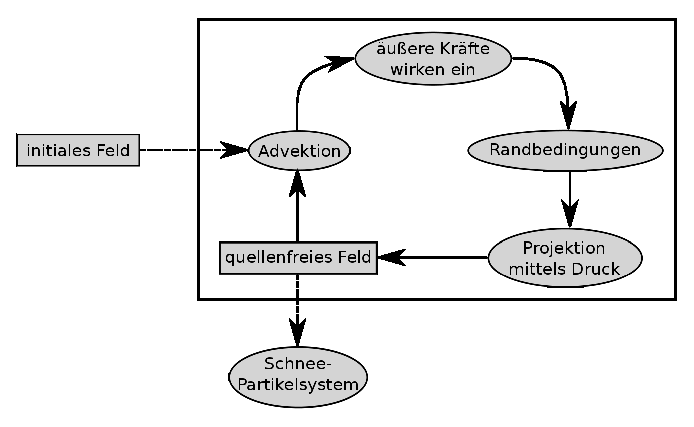
\includegraphics[width=10cm]{images/stam_loop_with_projection}
\caption{Die Simulationsschleife mit Projektion.}
\end{figure}

Definieren wir die einzelnen Schritte als Funktionen, ergibt sich im Pseudocode:

\begin{equation}
u^{t+\Delta t}
=
\PimiddyProjection(
	\PimiddyFormelText{advect}(
		\PimiddyFormelText{boundaries}(
			\PimiddyFormelText{externalforces}(
				u^t,
				\Delta t)),
		\Delta t))
\end{equation}

Im weiteren werden die Einzelschritte vorgestellt.

\subsection{Advektion}

Hier substanzielle Ableitung erklären? Oder schon früher bei den
Navier-Stokes-Gleichungen?

Wie bereits in der Erklärung der Navier-Stokes-Gleichungen angedeutet wird bei
der Advektion das Vektorfeld entlang seiner eigenen Geschwindigkeit
weiterbewegt. Im Folgenden gehen wir allgemeiner davon aus, dass eine beliebige
Größe $q(\vec{x},t)$ entlang des Vektorfelds $\vec{u}$ weiterbewegt werden soll,
also z.B. auch ein Temperaturwert oder die Rauchdichte.

Um diese Operation durchzuführen gibt es mehrere Ansätze. Der Intuitivste lässt
sich wie folgt beschreiben (\cite{Stam2003}):

Man stelle sich an jedem Gitterpunkt $\vec{i}=(i,j,k)$ ein Partikel mit
\PimiddyQuotes{Ladung} $q_{i,j,k}$. Durch das Vektorfeld würde das Partikel
um $\vec{u}_{i,j,k}$ verschoben und läge bei $\vec{p}=\vec{i}+\vec{u}_{i,j,k}$.
Somit läge es im Allgemeinen nicht mehr exakt auf einem Gitterpunkt, sondern
zwischen 8 Nachbarpunkten $n_i \in \PimiddyGanz^3, i \in \{1,\ldots,8\}$. Man bestimmt jetzt die
Distanz von $\vec{p}$ zu jedem der Nachbarpunkte:

\begin{equation}
d_i = \PimiddyNorm{2}{p - n_i}, i \in \{1,\ldots,8\}
\end{equation}

Diese $d_i$ dienen als Gewichtung, um die \PimiddyQuotes{Ladung} $q_{i,j,k}$
anteilig auf die Nachbarknoten aufzuteilen:

\begin{equation}
u_{n_i}' = u_{n_i}' + d_i \cdot q_{i,j,k}
\end{equation}

Dieses Verfahren ist intuitiv und einfach zu implementieren. Aber es ist
numerisch nicht stabil und führt zu Oszillationen (für eine genaue Betrachtung
sei auf die Literatur verwiesen).

Eine Alternative ist ein Ansatz mit finiten Differenzen wie in
\cite{Foster1997}. Dieser ist aber ebenfalls numerisch instabil.

Stam wählte einen anderen Ansatz, die sogenannte \emph{Methode der
Charakteristika}. Die Idee ist ähnlich zu der gerade vorgestellten, funktioniert
aber in die \PimiddyQuotes{umgekehrte Richtung}.

Wir betrachten wieder einen Gitterpunkt $\vec{i}=(i,j,k)$, nehmen diesmal aber
an, wir seien auf der Zeit-Achse im Punkt $t+\Delta t$, also bereits im nächsten
Zeitschritt. Das Partikel an Position $\vec{i}$ hat die Geschwindigkeit
$\vec{u}_{i,j,k}$. Rechnet man also auf der Zeitachse um $\Delta t$ zurück,
erhält man die \PimiddyQuotes{vorherige} Position des Partikels, nämlich
$\vec{i} - \Delta t \cdot \vec{u}_{i,j,k}$ \PimiddyFootnote{Hier wird nur ein
Schritt der Partikelflugbahn zurückverfolgt. Es gibt auch Methoden, die
mehrere Schritte verfolgen, diese sind aber aufwändig zu
implementieren.}. Es ergibt sich allerdings dasselbe
Problem wie bei dem vorher beschriebenen Ansatz: Diese Position liegt nicht
genau auf dem Gitter, sondern dazwischen.

Als Lösung interpolieren wir zwischen den 8 Nachbarwerten des verschobenen
Partikels und schreiben den entstehenden Wert in die Zelle $u'_{i,j,k}$. Dies
ist eine Operation, auf die Grafikkarten stark optimiert sind, und bei denen
traditionell Texturen hohe Performance erreichen können.

Natürlich kann es passieren, dass wir über den Rand des Simulationsbereiches
hinauslaufen. Hier können verschiedene Randbedingungen betrachtet werden.
Beispielsweise könnte man auf die gegenüberliegenden Seite des
Simulationsbereiches umbrechen (periodische Randbedingung), was in Stams Arbeit
getan wurde.

Alternativ kann man die Gitterpunkte, die am nächsten am Rand liegen, für die
Interpolation benutzen. Dies wurde in der Arbeit implementiert.

Weiterhin kann der zurückberechnete Vektor $\vec{i} - \Delta t u_{i,j,k}$ in
einem Hindernis landen. Man kann in diesem Fall einen Geschwindigkeitswert
von $(0,0,0)$ annehmen, was einem stationären Hindernis wie einem Gebäude
entspricht. Es ist aber auch möglich, ein weiteres Vektorfeld
$u_{\PimiddyFormelText{boundary}}$ zu verwalten, wo für jede Gitterzelle die
\emph{Geschwindigkeit} des dort vorhandenen Hindernisses notiert ist. Dies wurde
in \cite{Crane2007} umgesetzt. Für die Simulation in dieser Arbeit wurde von
unbeweglichen Hindernissen ausgegangen.

\PimiddyTodo{Hier noch Kommentar über die Stabilität (weil beim Interpolieren ja
	nichts \PimiddyQuotes{summiert} wird und so nichts größeres als das bisher dagewesene
	rauskommen kann. Außerdem steht in \cite{Foster}, dass man maximal 5
	Gridzellen weitergehen darf ohne zu viel Dissipation zu haben}

\subsection{Projektion}

\subsubsection{Lösung des Poissonproblems}

Um das Vektorfeld quellenfrei zu machen, muss folgende
\PimiddyBegriff{Poissongleichung} nach $p$ gelöst werden:

\begin{equation}
\PimiddyLaplace{p} = x
\end{equation}

wobei $x$ ein Skalarfeld ist. Es existieren zahllose Lösungsverfahren für so
eine Gleichung. Bei der Auswahl des Verfahrens muss beachtet werden, welches
sich gut auf der Grafikkarte umsetzen lässt. Hier haben sich mehrere sogenannte
\PimiddyBegriff{Iterationsverfahren} als günstig herausgestellt. Verfahren
dieser Art beginnen mit einer initialen Lösung (z.B. schlicht $p=0$) und nähern
sich dann in jedem Iterationsschritt weiter der eigentlichen Lösung an.

Betrachtet man große Felder, bieten sich \PimiddyBegriff{Mehrgitterverfahren}
an. Diese wurde bereits erfolgreich auf GPUs angewendet (siehe \cite{Bolz2002}),
sind allerdings untrivial zu implementieren, da intern ein zweites
Iterationsverfahren benötigt wird (der sogenannte Restriktionsoperator).

Simplere Iterationsverfahren sind SOR (umgesetzt in \cite{Saltvik2006}),
Gauss-Seidel-Re"-la"-xa"-ti"-on (umgesetzt in \cite{Stam2003}) und das
Jacobiverfahren (umgesetzt in \cite{Crane2007}, \cite{Harris2008},
\cite{Peschel2009}). Letzteres ist besonders einfach zu
implementieren und gleichzeitig hervorragend für die GPU geeignet.

\subsubsection{Das Jacobiverfahren}

Um das Jacobi-Verfahren zu veranschaulichen, betrachten wir das eindimensionale
Problem. Wir betrachten also kein diskretes 3D-Gitter, sondern eine Teilmenge
der ganzen Zahlen. Für die exakte Lösung $p$ des Poissonproblems muss an jeder
Stelle $p_i$ gelten (Randbedingungen werden später behandelt):

\begin{equation}
\label{stam_jacobi_onedimensional}
\frac{
	p_{i+1} -
	2 \cdot p_{i} +
	p_{i-1}
}
{
	2
}
=
x_i
\end{equation}

Angenommen wir hätten eine Anfangslösung $p^0$, z.B.
$p^0 = 0$. Dann können wir eine neue Lösung bestimmen,
indem wir \autoref{stam_jacobi_onedimensional} nach $p_i$ auflösen und dabei die
Nachbarwerte aus $p^0$ als Näherungen für die Nachbarn
in der exakten Lösung nehmen:

\begin{equation}
\label{stam_jacobi_onedimensional_iterative_solution}
p_i^1
=
\frac{
	x_i + p_{j+1}^{0} + p_{j-1}^{0}
}
{
	2
}
\end{equation}

Im nächsten Iterationsschritt berechnet man dann $p_i^2$ mit Hilfe von $p_i^1$,
usw., bis man nahe genug an die exakte Lösung herangekommen ist. In der Praxis
sind mindestens 20 Iterationen nötig, da das Verfahren sehr langsam konvergiert.

Eine leichte Konvergenzverbesserung erreicht man, indem man die rechte Seite von
\autoref{stam_jacobi_onedimensional_iterative_solution} nicht direkt als neue
Lösung nimmt, sondern zwischen der bisherigen Lösung und der neue Lösung mit
einem Gewichtungsfaktor $\omega$ interpoliert:

\begin{align}
\overline{p}_i^{n+1}
&=
\frac{
	x_i + p_{j+1}^{n} + p_{j-1}^{n}
}
{
	2
} \\
p_i^{n+1}
&=
(1-\omega) \cdot p_i^n + \omega \cdot \overline{p}_i^{n+1}
\end{align}

Dieses Verfahren wird \PimiddyBegriff{gewichtete Jacobi-Iteration} genannt. In
der Praxis hat sich ein Faktor von $\omega=\frac{2}{3}$ als günstig erwiesen.

\subsubsection{Randbedingungen}

Auch beim Druck müssen Randbedingungen betrachtet werden. Dies betrifft wiederum
den Rand der Simulation sowie Hinderniszellen.

Der Rand der Simulation soll so geartet sein, als wäre die Simulation an den
Seiten \PimiddyQuotes{offen}. Das Fluid soll am Simulationsrand nicht abprallen,
sondern sich dorthin weiter ausbreiten (outflow boundary conditions
\PimiddyTodo{verifizieren und übersetzen}). Um dies anzunähern verändern wir vor
dem Projektionsschritt das Geschwindigkeitsfeld so, dass die
Geschwindigkeitswerte am Rand denen \PimiddyQuotes{neben dem Rand} entsprechen.
So entsteht bei der Bildung des Drucks kein Unterschied zu den Nachbarzellen und
bei der Gradientbildung im nächsten Schritt ergibt sich $0$.

Für Hindernisse im Simulationsbereich wollen wir sogenannte
\PimiddyBegriff{free-slip}-Randbedingungen umsetzen. Wie der Name andeutet
erzwingen diese Randbedingungen, dass sich das Fluid (tangential) entlang des
Hindernisses bewegen kann aber nicht in das Hindernis hineinfließen darf.
Ist $\vec{n}$ die Normale an einem Punkt des Hindernisses und
$\vec{u}_{\PimiddyFormelText{Hindernis}}$ die Geschwindigkeit des Hindernisses,
dann muss im Geschwindigkeitsfeld des Fluids gelten:

\begin{equation}
\vec{u} \cdot \vec{n} = \vec{u}_{\PimiddyFormelText{Hindernis}} \cdot \vec{n}
\end{equation}

Da wir im weiteren $\vec{u}_{\PimiddyFormelText{Hindernis}}=0$ annehmen gilt:

\begin{equation}
\vec{u} \cdot \vec{n} = 0
\end{equation}

Ohne Herleitung stellen wir fest, dass sich dies sehr einfach in den
Jacobi-Algorithmus integrieren lässt. Wir testen für jede Nachbarzelle der
aktuellen Zelle, ob diese von einem Hindernis belegt ist. Ist dem so, ersetzen
wir den Druckwert durch den der aktuellen Zelle. Wir ignorieren also Nachbarn,
die von Hindernissen belegt sind.

Da der Jacobi-Algorithmus die Projektionsgleichung nur annähernd löst,
erzwingen wir am Ende die Randbedingungen für die Voxel, die an Hindernisse
angrenzen, explizit.

\subsection{Äußere Kräfte}

\subsubsection{Gravitation}

Zu den äußeren Kräften gehört zu allererst die \emph{Gravitation}. Diese lässt
sich sehr einfach ausdrücken:

\begin{equation}
F_g = \Delta t (0,-9.81,0)
\end{equation}

\subsubsection{Auftrieb}

\PimiddyTodo{Auftrieb allgemein und konkret mit Buissnesq erklären}

\subsubsection{Wirbelstärkenerhaltung}

\PimiddyTodo{Vorticity Confinement erklären.}


\bibliographystyle{plain}
\bibliography{mendeley_bibliography}

\end{document}
